\subsection{Pretraining}
\label{sec:app-pretrain}

In pretraining, \pace\ beats both the AdamW and \ema\ baselines under every
learning-rate schedule, and the best pullback strength is the same under all of
them. The figures below show the full pullback-strength sweep on GPT-2-124M
(trained from scratch on \texttt{FineWeb} at the Chinchilla-optimal budget), as
the mean over three seeds $\{0,1,42\}$.

\paragraph{Multi-seed pullback-strength sweep across schedules.}
\Cref{fig:appendix_pretrain_csweep} sweeps the pullback strength $c$ under all
three schedules (the AdamW and best-$\kappa$ \ema\ baselines are the two leftmost
ticks). Two things stand out. First, at its optimum \pace\ beats both baselines
under every schedule, and the improvement holds across a band of pullback
strengths ($10^{-3}\le c\le 3{\times}10^{-3}$)---wider still under WSD and cosine.
Second, the optimum is the same ($c\approx 3{\times}10^{-3}$) under all three
schedules, so the choice of $c$ transfers. WSD with \pace\ is best overall
($3.507\pm0.006$, below the constant-LR optimum of $3.537\pm0.004$ by several
times the seed spread), and \pace\ at a constant learning rate comes within
$0.006$ of AdamW under WSD ($3.537$ vs.\ $3.531$) with no schedule at all.
\Cref{fig:appendix_pretrain_csweep_kappa} resolves the same grid by the EMA
power $\kappa$ (at seed $42$) and shows a basin around the optimal $c$ at every
$\kappa$.

\begin{figure}[ht]
  \centering
  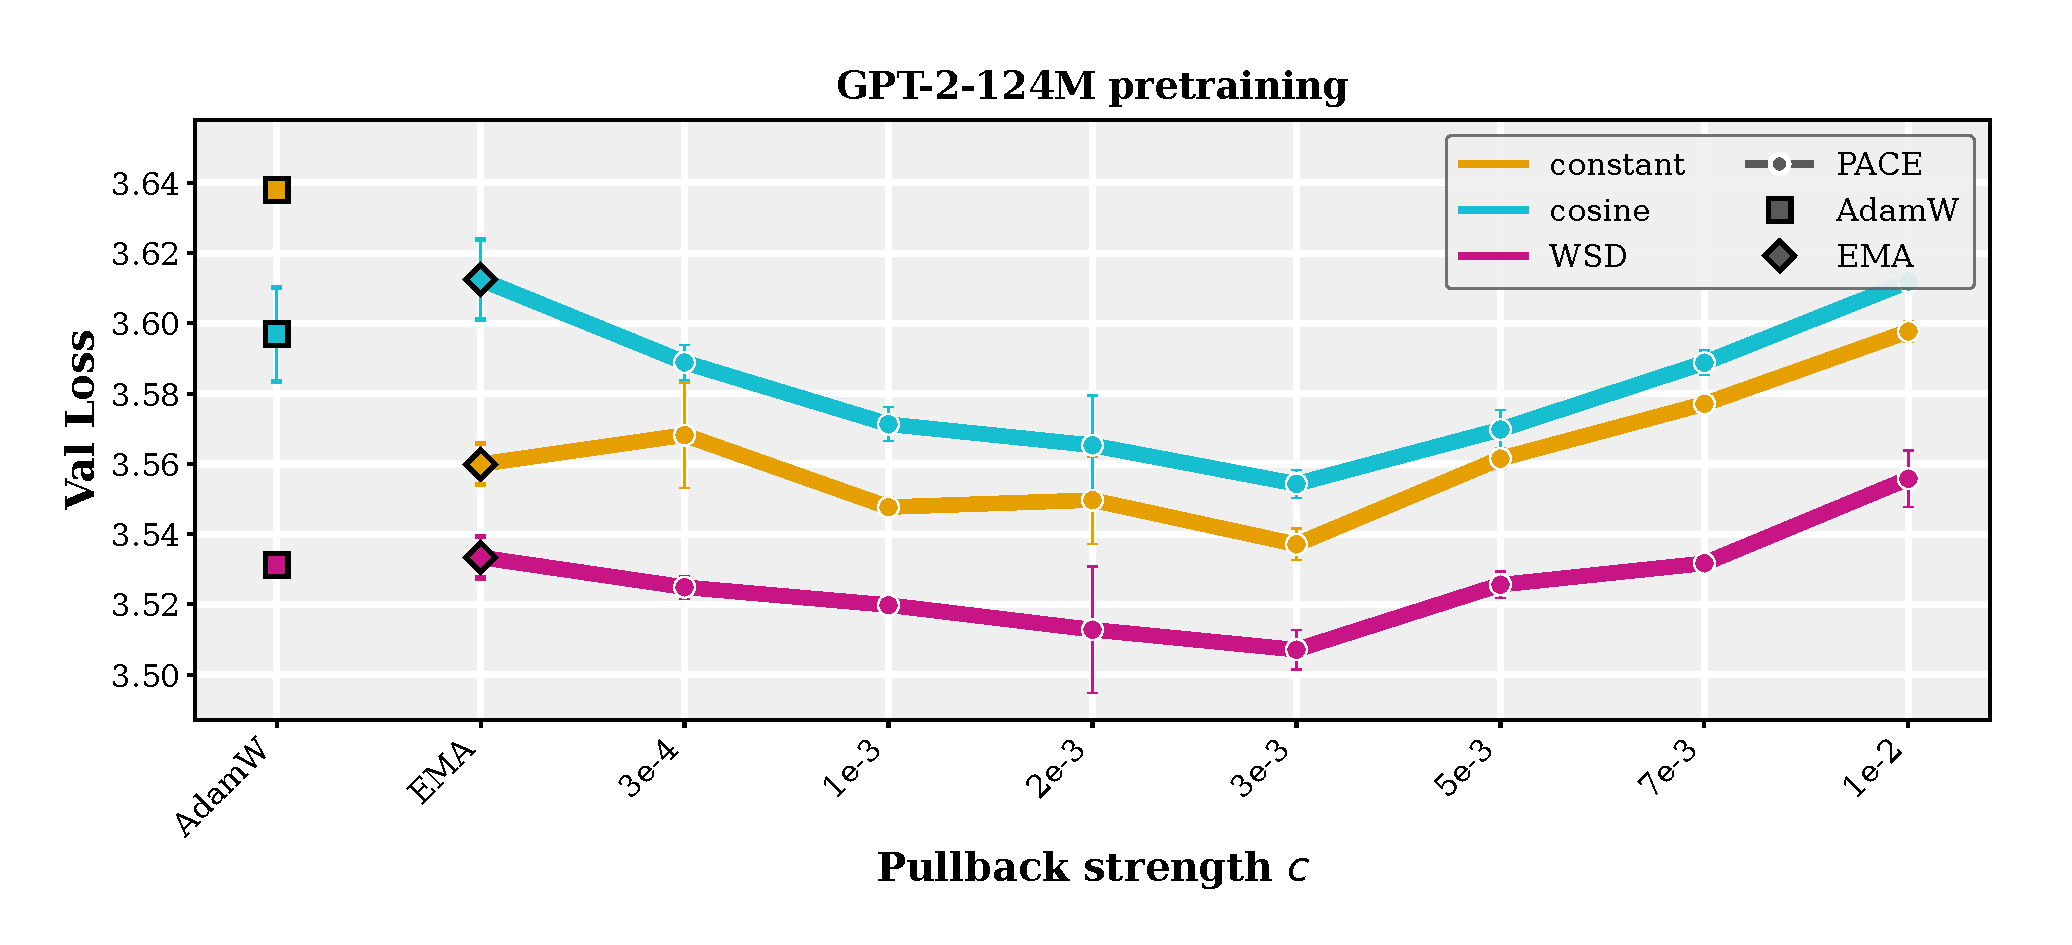
\includegraphics[width=0.676\textwidth]{figures/fig_appendix_pretrain_csweep.pdf}
  \caption{\textbf{Multi-seed pullback-strength sweep across learning-rate
  schedules} on GPT-2-124M pretraining. Mean returned-model validation
  cross-entropy with seed-to-seed standard deviation, comparing \pace\ to the
  AdamW and \ema\ baselines under each schedule. \pace\ improves on both
  baselines under every schedule, by more than the seed-to-seed variation.}
  \label{fig:appendix_pretrain_csweep}
\end{figure}

\begin{figure}[ht]
  \centering
  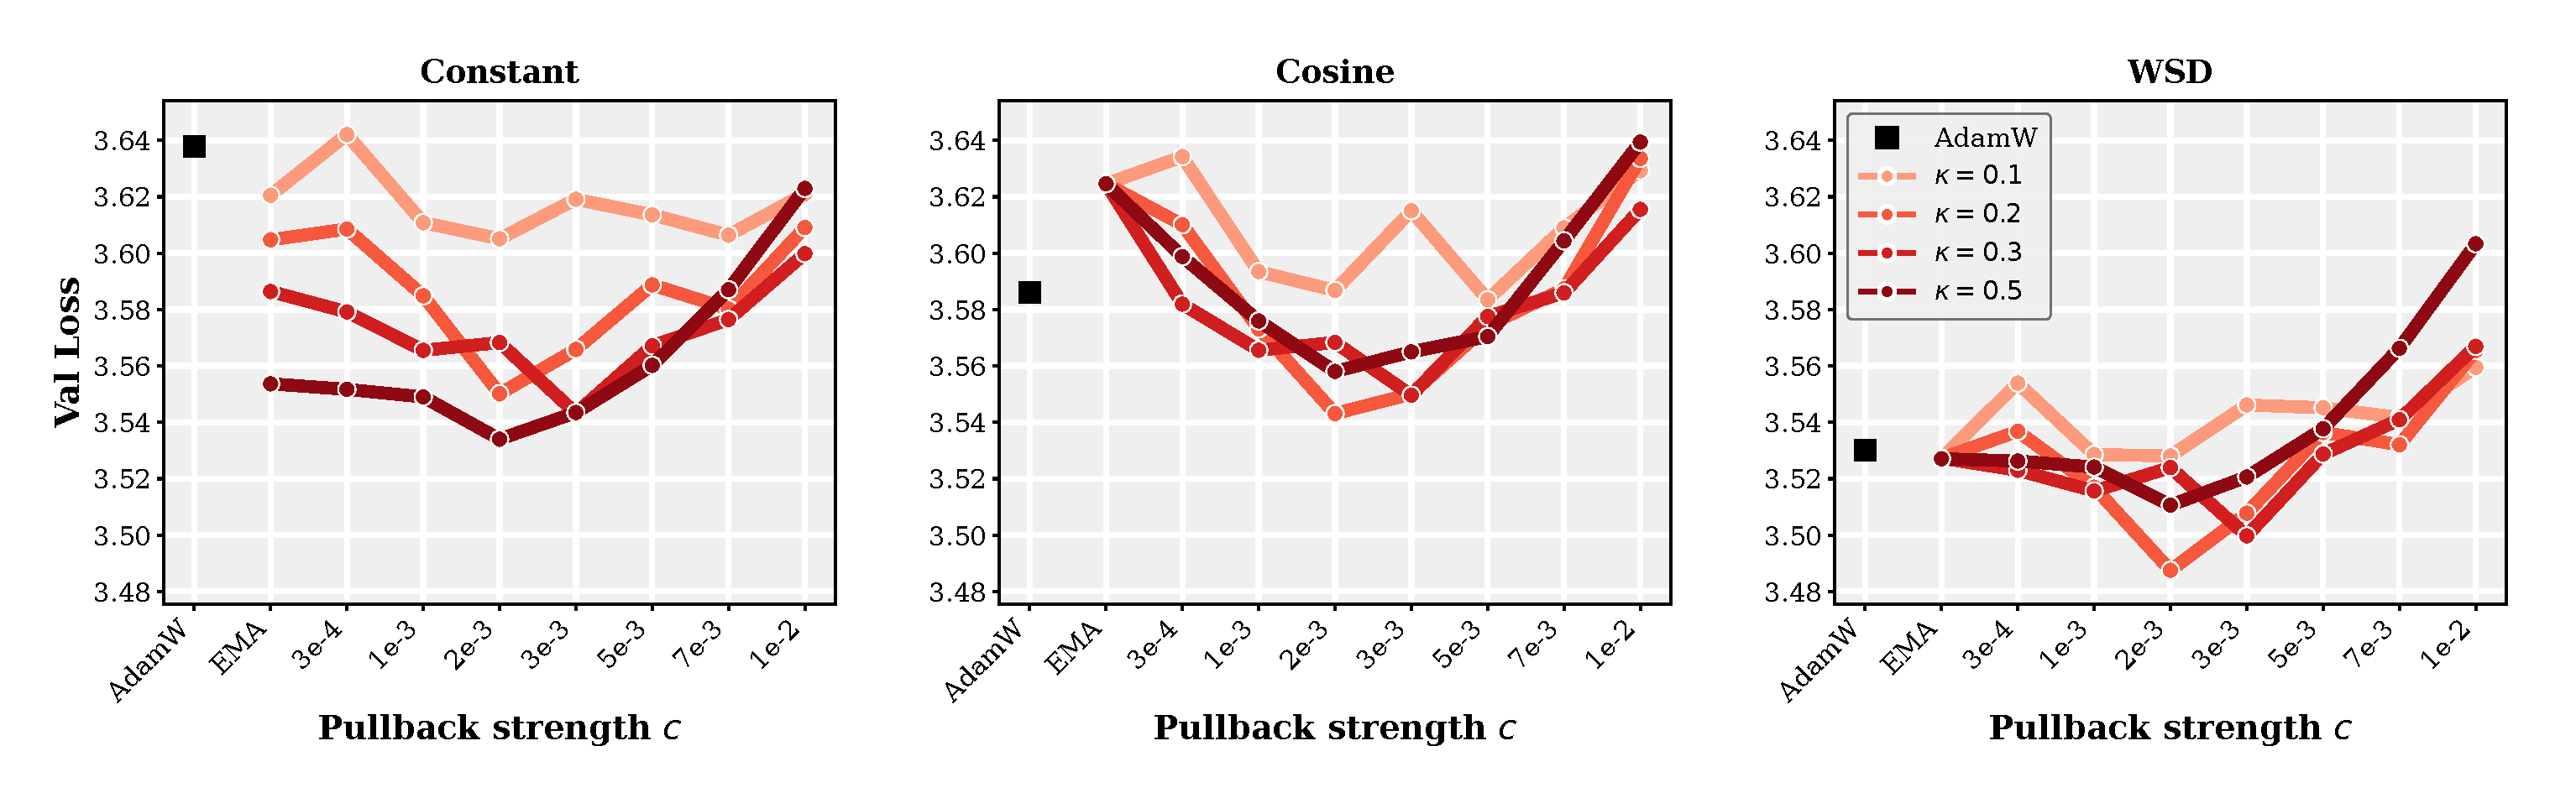
\includegraphics[width=\textwidth]{figures/fig_appendix_pretrain_csweep_kappa.pdf}
  \caption{\textbf{Pullback-strength sweep resolved by EMA power} on
  GPT-2-124M pretraining (seed $42$), under a constant learning rate
  (\textbf{left}), cosine decay (\textbf{middle}), and WSD (\textbf{right}). A
  basin spanning $c\approx 2$--$3{\times}10^{-3}$ appears at every $\kappa$
  under every schedule.}
  \label{fig:appendix_pretrain_csweep_kappa}
\end{figure}
